    %
    \documentclass[twoside,a4paper]{refart}
    \usepackage[T1]{fontenc}
    \usepackage{ae} 
    \usepackage{makeidx}
    \usepackage{ifthen}
    \usepackage{graphicx}

    \DeclareRobustCommand\cs[1]{\texttt{\char`\\#1}}
    \def\bs{\char'134 } 
    \newcommand{\zB}{z.\,B.}
    \newcommand{\dH}{d.\,h.}  

    \title{HamerMEMS Field Guide for the End-User}
    \author{
    Martin Binder \\
    Benedikt Holler \\
    Andreas M\"uller }
    \date{\today}
    \emergencystretch1em 
    \makeindex

    \setcounter{tocdepth}{2}
    \settextfraction{0.7}

    \begin{document}
    \maketitle

    \tableofcontents

    \newpage


    %%%%%%%%%%%%%%%%%%%%%%%%%%%%%%%%%%%%%%%%%%%%%%%%%%%%%%%%%%%%%%%%%%%%

    \section{Introduction}

    \subsection{Motivation}
The Hammer EMS (Energy Management System) described in this manual seeks to give users insight into the performance of computing devices within a system. \\
That performance is represented by and encapsulated within a set of Key Performance Indicators (KPIs), including for example energy demand, memory usage and network throughput. \\
For the sake of convenience, the interface can be accessed through any preferred web browser. \\
Please contact your system administrator before starting work with the EMS. You will need a link to the Frontend webpages as well as login credentials. \\
Please note that only Mozilla Firefox and Google Chrome are supported by this EMS.

    %%%%%%%%%%%%%%%%%%%%%%%%%%%%%%%%%%%%%%%%%%%%%%%%%%%%%%%%%%%%%%%%%%%%


    \section{Login}
    \label{login}
    \index{Login}

    \subsection{Registration}
    \index{Registration}
Since you're reading this User Manual, you probably received a registration E-mail. \\
In this mail, you will find a username and a password. \\
Please check whether you have a stable internet connection, as well as access to the University network (or to the network which the EMS was set up on). \\ 
You can find a guide how to access the universtity intranet with OpenVPN under the following link:\\http://www.zim.uni-passau.de/en/dienstleistungen/netzwerk-und-server/network-access/openvpn/) \\
    \subsection{Login}
  	Enter  the link you were given by your administrator for login into 	your web browser's navigation bar. \\
    Enter your user name and password into the respective fields, then 		click on "Login". \\
    If the login has been successful, the main page will load. \\
    Otherwise, you will remain on the Login page. Please confirm 			whether you entered your credentials correctly. If you forgot your 		password, you may refer to section \ref{forgot}.
    \index{Login}
    \subsubsection{Logout}
    \index{Logout}
    You can log out of the system from any page on the Frontend. Simply click on the Profile Icon in the top right corner of the screen: \\
  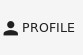
\includegraphics[width=50px]{profile.jpeg} \\
  Then, click "Log Off": \\
  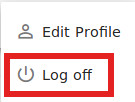
\includegraphics[width=50px]{logoff.jpeg} \\
    Please make sure you log out every time you are done working with the EMS in order to prevent unauthorized access by third parties.
  
    \section{Profile}
    \label{profile}
    \index{Profile}
    In the top right corner, you can find this icon: \\
    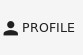
\includegraphics[width=50px]{profile.jpeg} \\
    Clicking on it and then clicking on "Edit Profile" will open your profile, which looks like this: \\
    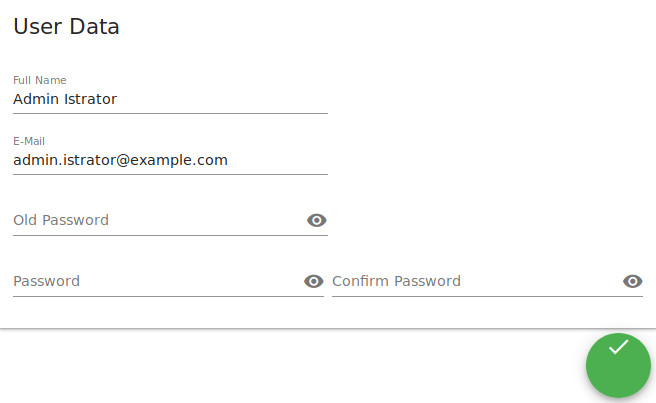
\includegraphics[width=\linewidth]{userprofile.jpeg} \\
    \begin{itemize}
    \item[Full Name:] Here you will find your name. You can change your name yourself, though remember that it mustn't be empty.
    \item[Email:] Your E-mail address on which you receive mails sent from the EMS. Be careful when changing your e-mail address, since you need it in case you forget your password.
    \item[Changing your password:]
    To change your password, first enter your current password. If you forgot your current password, refer to section \ref{forgot}. \\
    Then, type in your new password, confirm it in the second box, and click the green check button. A popup message will confirm if your password was changed successfully.
\end{itemize}     
    
    \section{Navigation}
    \label{navi}
    \index{Navigation}
    Here's an overview of all navigation elements you can find within the EMS software: \\
    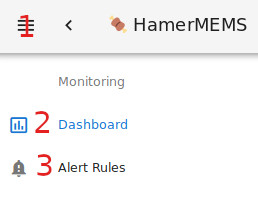
\includegraphics[width=100px]{navigation1.jpeg} \\
    (1) Hides and shows the navigation sidebar. \\
    (2) Navigates to the dashboard page to display KPI graphs. \\
    (3) Navigates to your Alert Rules. \\
    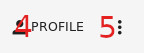
\includegraphics[width=75px]{navigation2.jpeg} \\
    (4) Opens a submenu where you can access your user profile and log off the EMS. \\
    (5) Hides and shows the node sidebar for the dashboard. Only has a function while you are on the dashboard page. \\
    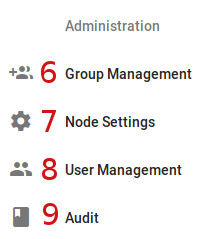
\includegraphics[width=100px]{navigation3.jpeg} \\
    (6) Navigates to the group management page where user groups can be added, deleted and changed. (Admin only) \\
    (7) Navigates to the node overview page where nodes can be added, deleted and changed. (Admin only) \\
    (8) Navigates to the user overview page where users can be added, deleted and changed. (Admin only) \\
    (9) Navigates to the Audit Log, where authorized actions are kept track of. (Admin only)
    \section{Monitoring -> Dashboard}
    \subsection{All functions of the dashboard}
    At first, the monitoring page is empty. To display graphs, click on the three dots in the top right corner. \\
    Next, click on the names of nodes you want to display graphs for (if no nodes appear in this place, please contact your administrator). \\
    Once nodes are selected, for each node, you can decice whether you want data to be displayed live or within a specific time window. \\
    To display live data, click on "live", then you may enter the amount of minutes you want to be displayed (default is 60). \\
    To display a specific time window, click "history", then enter start and end dates. Note that these must be \emph{exactly} in the format YYYY-MM-DD,hh:mm:ss:xxx (year, month, day, hours, minutes, seconds, milliseconds respectively) and that you only may only use numbers. For example, if you want to set a date to the third of February of 2019, at 12:30, enter "2019-02-03,12:30:00:000".
     

    \section{Alert}
    To access the alert page, click on alert rules in the navigation bar.
    On the alert page you find an overview of alert rules. If it is your first time accessing this site, the list of alert rules should be empty. \\
    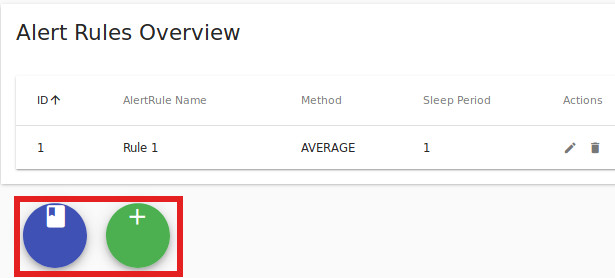
\includegraphics[width=\linewidth]{alertoverview.jpeg} \\
    At the bottom of the page, you see two buttons, the blue one will bring  you to the Alert Notifications History, the green one will bring you to +the alert creation page.    
    
    \subsection{How to create alerts}
    Click on the green button with the "+". This will open an alert page,
    where you can set the name of the new alert rule and chose the method when an alert rule shall be triggered.
    Here's a description what the different methods do:
    \begin{itemize}
    \item[Average:] Calculates the average value of the received KPIs from a
    node over a a set time period, and notifies
    you, if the average crosses the threshold.
    \item[Median:] Checks if more than half of the received values of the
    selected KPI surpass the threshold.
    \end{itemize}
    When you are finished, you have to save the new alert rule. Saving the new alert rule should bring you to the alert rule page. In the overview should now be a new alert rule listed. \\
    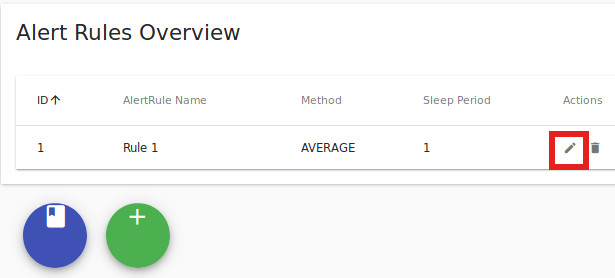
\includegraphics[width=\linewidth]{alertedit.jpeg} \\
    Click on the edit symbol on the new alert rule. Now you should be on the page where you left before you clicked on save, though now you can click on next.\\ \\
    On this page, you can choose different KPIs that you want to monitor.
    You can now set the threshold of the different KPIs (don't forget to set the threshold!). Do not select the same KPI for monitoring twice here! \\
    With the leq checkbox you can decide if you want to be notified if the value surpasses or falls below the threshold (leq: lower or equal).\\
    If you accidentally selected a KPI, you can remove the KPI by clicking on the delete button (bin symbol). \\
    Once you have chosen your KPIs settings, you can click on next.
    Now you can decide which nodes you want to attach this alert rule to.
    Clicking on the text field should list all nodes that are available to you (If no nodes are listed, you are in no group; contact the Administrator and ask them to put you into a group).\\
    Once you have the nodes selected, click on "update" to save the changes on your alert rule.
    
    \subsection{How to see your notifications}
    On the alert page, there is still this blue button: \\
    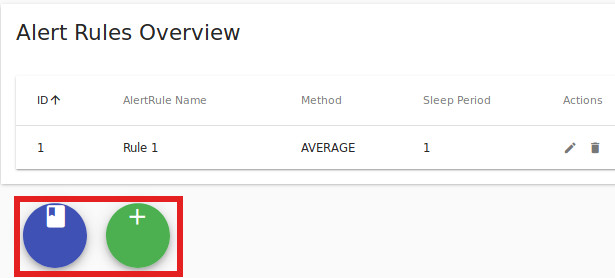
\includegraphics[width=\linewidth]{alertoverview.jpeg}
    you will get to the alert notification history page. You can view all of your notifications here.\\
    You can remove notification if you click on delete.

\section{Group Management}
Note that you only have access to the Group Management if you are an admin or a privileged user!\\
In the context of our EMS, a user group is merely a way to assign users to nodes. Users can only see nodes and assign alert rules to nodes they have access to through a user group.\\ \\
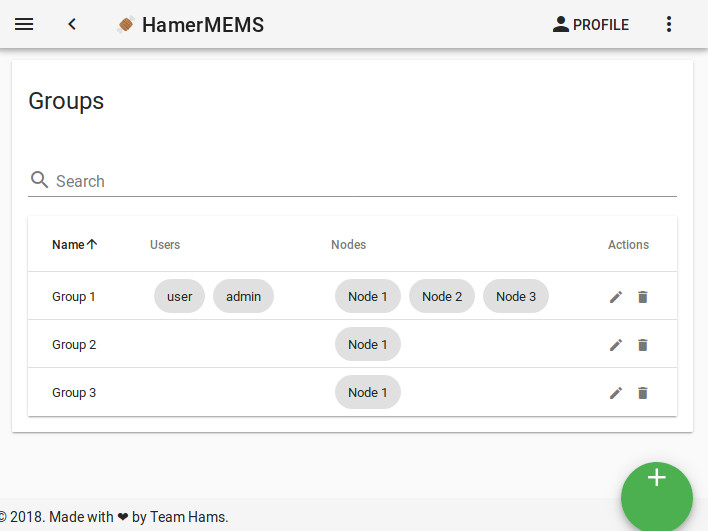
\includegraphics[width=\linewidth]{groupmanagement.jpeg} \\  \\
Using the search bar, you can search for specific groups by name.\\
By clicking the pencil icon next to a node, you can edit that group: \\
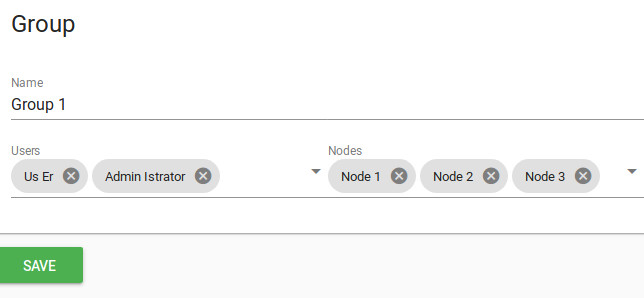
\includegraphics[width=\linewidth]{groupedit.jpeg} \\
Under "Name", you can directly type in a new name if you wish to rename the group. \\
Under "Users" and "Nodes", you can remove units from the group by clicking the X next to them, and add more by clicking the down arrow and selecting them from a list. \\
If you are done editing the group, click "Save".\\ \\
By clicking the bin icon next to a group, you can delete that group. You will be asked once more if you are sure you want to delete it. \\
Be careful, once you delete a group there is no way to get it back. \\ \\
By clicking the green button with the "+", you can add a new group: \\
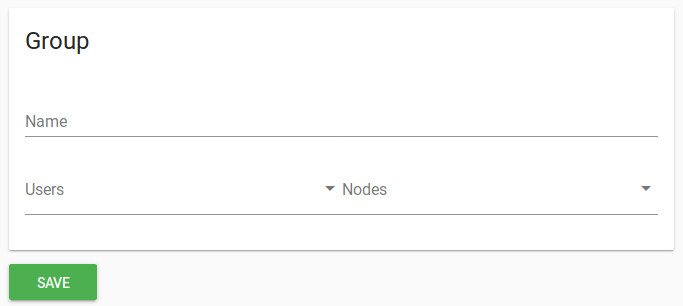
\includegraphics[width=\linewidth]{groupadd.jpeg} \\ \\
Under "name", you must enter a name for your group. Under "Users" and "nodes", you can select units that should be assigned to your group. Note that both Users and Nodes \emph{must not} be empty!
\section{Node Management}
Note that you only have access to the Node Management if you are an admin! \\
This page gives you an overview of the nodes connected with the EMS, their names, and their send interval. The send interval is the time period between separate KPI messages from that node (e.g. if a node has a send interval of 20, that node sends KPI messages each 20 seconds). \\ \\
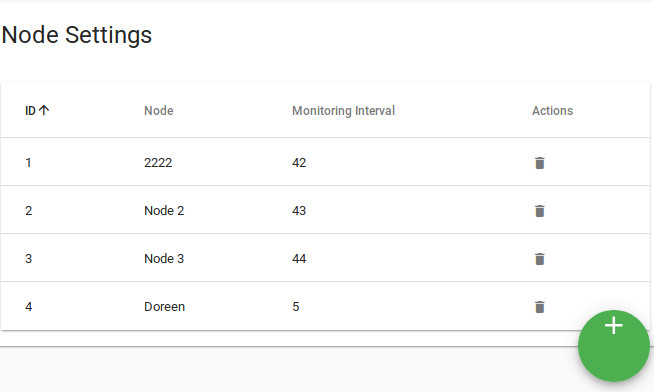
\includegraphics[width=\linewidth]{nodeoverview.jpeg} \\ \\
If you want to change any of these information, simply click on it. A prompt will open up where you can enter the new data. Note that neither the name or send interval can be empty or zero. \\ \\
By clicking the bin icon next to a node, you can delete that node. You will be asked once more if you are sure you want to delete it.  \\
Be careful, once you delete a node there is no way to get it back, unless you register it again. \\ \\
By clicking the green button with the "+", you are taken to a page with a registration pin: \\ \\
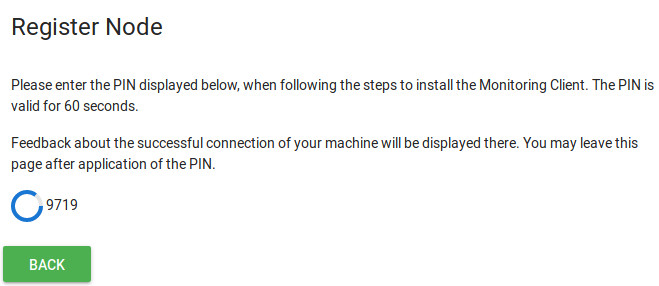
\includegraphics[width=\linewidth]{nodepin.jpeg} \\ \\
Please refer to the admin manual on how to register a new monitoring client on a node using this pin.
\section{User Management}
Note that you only have access to the User Management if you are an admin! \\ 
This page gives you an overview of all users within the system. \\ \\
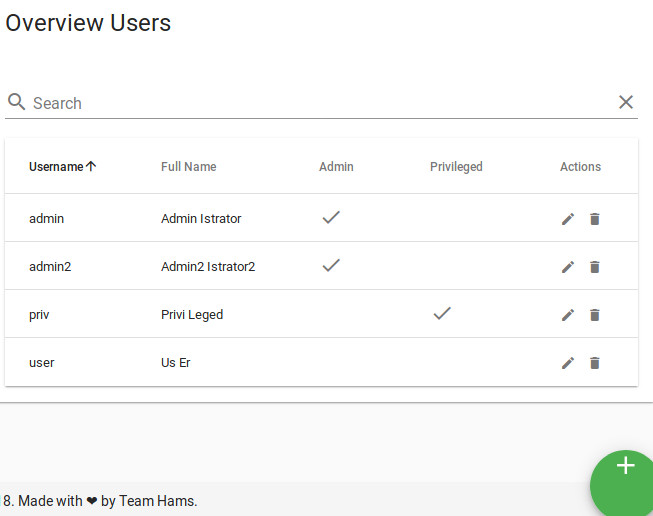
\includegraphics[width=\linewidth]{useroverview.jpeg} \\ \\
Using the search bar, you can search for specific users by name.\\
By clicking the pencil icon next to a user, you can edit that user: \\
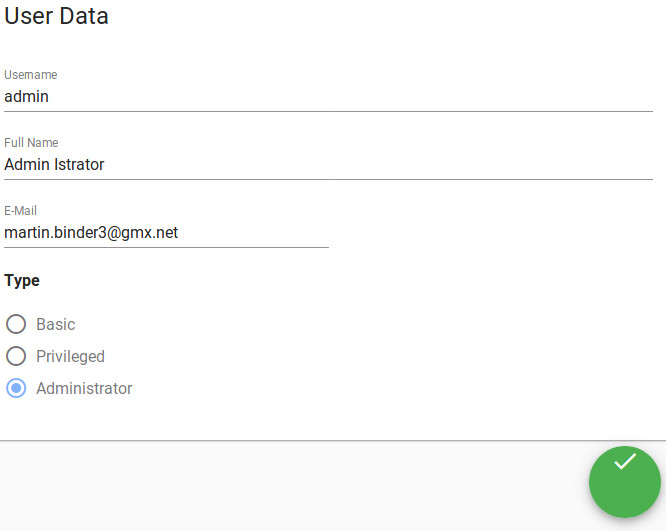
\includegraphics[width=\linewidth]{useredit.jpeg} \\ \\
Under "Username", "Full Name", and "E-mail", you can change that information for the selected user. Note that you can not change a user's password here, that is instead done in the user's profile. \\
You can also set a user's type here. \\
If you are done with your changes, click the green button with the tick. \\ \\
By clicking the bin icon next to a user, you can delete that user. You will be asked once more if you are sure you want to delete it. \\
Be careful, once you delete a user there is no way to get it back. \\ \\
By clicking the green button with the "+", you can add a new user: \\ \\
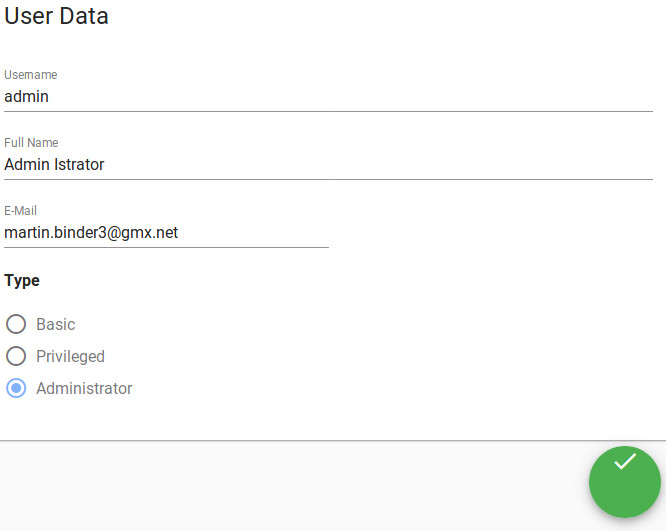
\includegraphics[width=\linewidth]{useredit.jpeg} \\ \\
This screen is the same when editing a user. You can enter the new user's information in the corresponding fields and set its type. Once the user is created, they will receive a mail on the address you entered; from there, they can go through the password set process.
\section{Audit Log}
Note that you only have access to the Audit Log if you are an admin! \\
This page gives you an overview of crucial actions that were performed within the EMS. \\ \\
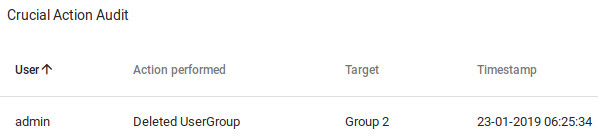
\includegraphics[width=\linewidth]{audit.jpeg} \\ \\
"User" displays the user who performed the action. \\
"Action performed" gives a short description of what has been done. \\
"Target" shows what the target of the action was, e.g. a node or a user group. \\
"Timestamp" shows when the action was performed.

\section{Glossary} 
In this section, important expressions and phrases shall be explained.
\begin{itemize}	
	\item[Admin/Administrator:] A user who has access to all aspects of the EMS, including User, Node and Group management.
	\item[Audit Log:] A log that lists all crucial actions that were done by users in the frontend.
	\item[Backend]: The part of the EMS that handles the most of the program logic and databases. Has direct contact with both the frontend and monitoring client.
	\item[Chrome:] A commonly used web browser developed by Google that works on most operating systems.
	\item[EMS:] Energy Monitoring System. A system used to monitor energy consumption and performance of a device. The system described in this document is an EMS.
	\item[Firefox:] A commonly used web browser developed by Mozilla that works on most operating systems.
	\item[Frontend:] The part of the EMS that can be accessed through web browsers.
	\item[KPI:] Key Performance Indicator. A unit that directly describes the efficiency of something in a certain aspect. For example, disk throughput in Kbit/s describes how much data is transfered through a disk.
	\item[Monitoring Client/MC:] Part of the EMS that is installed on a node.
	\item[Node:] A electronic device which is connected to the EMS, that has monitoring software installed and is sending KPIs.
	\item[Privileged User:] A user who has the rights to manage user groups. Not to be confused with an admin.
	\item[User:] Anybody who uses this system.
	\item[User Group:] In the context of the EMS, a way to connect users and nodes. A regular user can only see nodes if they are in a group which has that node assigned to it.
	\end{itemize}
    \end{document}